

\subsection{Описание предметной области <<Индивидуальный учет рациона поголовья коров>>}
Рацион --- это порция и состав пищи или корма на определённый срок. От ценности рациона для коров зависят рубцовое и послерубцовое пищеварение, потребление корма, здоровье, продуктивность и репродуктивная функция. Учет может осуществляться индивидуально по каждому животному или по группе животных. Корова --- крупный рогатый скот молочного направления. Для каждой коровы фиксируются характеристики: инвентарный номер (бирка или чип), порода, вес, возраст, физиологическое состояние (дойная или сухостойная), этап лактации и суточный удой. Суточный удой --- это количество молока (в кг, л), получаемое от сельскохозяйственных животных (коров, овец, кобыл и др.) за учётный период. Для оценки питательности кормов определяют в них общие элементы питания: белки, жиры, углеводы, витамины и минералы; макроэлементы и микроэлементы. \cite{косарева2020} Структурность корма определяется физической формой ингредиентов и содержанием плохо перевариваемых в рубце компонентов сырой клетчатки, в том числе балластных веществ (прежде всего лигнина).
\cite{ганущенко2019}
\begin{comment}
От размера частиц ингредиентов зависит качество их смешивания, потребление корма и эффективность его переваривания. От количества клетчатки в рационе зависит состояние здоровья коров, величина удоя и качество молока. 

    У жвачных животных балластные вещества не перевариваются ферментами самой коровы, но служат субстратом для микроорганизмов рубца. В результате микробной ферментации образуются летучие жирные кислоты --- основной источник энергии.
    Кроме того, клетчатка выполняет важные функции: регулярное очищение кишечника, связывание в ЖКТ токсинов и выведение их из организма. Вследствие недостаточной наполненности рациона балластными веществами ухудшается потребление кормосмеси на 10–20\%, снижается эффективность использования энергии и протеина на 5–10\% и продуктивность коров на 10–20\%. При чрезмерной наполненности рациона балластными веществами также сокращается продолжительность и активность жвачки, уменьшается выделение слюны, а значит, и буферная емкость рубца. Максимального потребления и оптимального переваривания всех компонентов рациона достигают путем поддержания основных параметров кормосмеси на нормальном уровне (влажность — около 50\%, концентрация сырого протеина в сухом веществе — 17–19\%, сырой клетчатки — 16–18\%). Высокопродуктивные дойные коровы должны ежедневно получать около 400 г структурной сырой клетчатки или 1100–1200 г нейтрально-детергентной клетчатки на каждые 100 кг живой массы. Нейтрально-детергентная клетчатка --- современный показатель, включающий целлюлозу, гемицеллюлозу и лигнин, который показывает общее содержание клетчатки. Сырой клетчатки много в соломе --- 40–45\% в сухом веществе, и сене --- 30–35\% в сухом веществе, и мало в зерне и корнеклубнеплодах --- 0,4–2\% в сухом веществе. Чем больше клетчатки, тем ниже питательность корма. В молодых злаковых травах концентрация сырой клетчатки составляет всего 14–16\% в сухом веществе, а после цветения ее уровень повышается до 34–35\%. Немецкие ученые установили, что в кормосмесях для крупного рогатого скота на долю структурной сырой клетчатки травяных кормов должно приходиться 60–65\% от всей клетчатки в рационе, а неструктурной сырой клетчатки, которая входит в состав концентратов и корнеклубнеплодов, --- 35–40\%. \cite{ганущенко2019}

    Люцерна, нут, чечевица, эспарцет, соя и люпин богаты микроэлементами, а сено из злаковых трав, сахарная свекла и зерновые --- бедны. При йододефиците у животных диагностируют такую патологию, как гиперплазия щитовидной железы (эндемический зоб). При
этом подавляется синтез белка в организме и замедляется основной обмен. В организм с кормом должно поступать оптимальное количество йода --- 0,2–0,5\% от общего объема сухого вещества рациона. У телок в возрасте 1–12 месяцев потребность в йоде составляет 0,3–0,7 мг в сутки, у коров в первой половине лактации --- 6–7,5 мг (в зависимости от живой массы). Для профилактики йододефицита лактирующим коровам необходимо давать корм, содержащий в 1 кг сухового вещества 0,4 мг йода. При нехватке меди пропадает аппетит, снижается потребление корма, что ведет к истощению и нарушению воспроизводительной функции. Скармливание пастбищных трав, богатых медью, но бедных молибденом, служит
причиной отравления животных медью. Молибден играет важную роль в обменных процессах, в частности в переваривании клетчатки бактериями рубца. При дефиците молибдена ухудшается белковый и жировой метабо-
лизм, деформируется скелет и происходят сбои в репродуктивной системе. Вследствие потребления кормов, содержащих избыточное количество молибдена, у коров развивается анемия
и снижается продуктивность. Марганец необходим для нормального функционирования центральной нервной системы, роста и развития молодняка. Цинк входит в состав гормонов и ферментов, участвует
в окислительно-восстановительных процессах. Вследствие дефицита цинка снижается потребление рационов и замедляется
рост животного. При поступлении цинка в повышенных дозах
(например, при поедании корма, хранившегося в оцинкованных емкостях) нарушается рубцовое пищеварение и возникают
запоры. Избыток цинка в кормах вызывает отравление.
Животным нужен и селен. Недостаток его в пастбищных
травах --- основная причина широко распространенных патологий крупного рогатого скота.
Кобальт --- жизненно необходимый элемент. Он входит в со-
став кобаламина --- витамина В12. При кормлении жвачных травами, произрастающими на почвах, бедных кобальтом, в преджелудках замедляется синтез витамина В12. В результате нарушается протекание обменных процессов, снижаются молочная
продуктивность и устойчивость организма к инфекционным
и паразитарным заболеваниям. Акобальтоз чаще диагностируют у высокоудойных коров.
Фтор играет важную роль в образовании костной ткани
и формировании зубной эмали, а также в фосфорно-кальциевом и углеводном обмене. Содержание фтора в костях и зубах взрослых здоровых коров варьирует в пределах 0,1–0,7\%.
В нормальных дозах фтор предотвращает развитие кариеса
и способствует заживлению переломов. Повышенный уровень
фтора оказывает на организм токсическое действие. У живот-
ных пропадает аппетит, что в конечном итоге приводит к исто-
щению. Максимальная доза фтора для крупного рогатого ско-
та не должна превышать 100 мг на 1 кг сухого вещества корма.
\end{comment} 
Для кормления коров используют различные виды кормов. Зелёные корма: трава пастбищ, скошенная зеленая масса разнотравья, бобовых культур, водоросли, овощи, ботва; грубые корма: солома, сено; сочные (объемистые) корма: сенаж, зерносенаж, овощи, силос, корнеплоды, другая растительная масса с высокой влажностью; концентрированные корма: комбикорм, зерновые смеси, жмыхи и шроты, премиксы. Примерная структура рациона для дойного поголовья должна составлять: 50\% --- сочные корма (силос, травы), 20\% --- грубые корма (сено, сенаж), 30\% — концентраты. Также животные должны быть постоянно обеспечены водой температурой не ниже 9-10°C в свободном доступе.
Потребность в  микроэлементах (железе, меди, цинке, марганце, йоде, кобальте) животные удовлетворяют за счет поедания основных кормов. 
Помимо микроэлементов, в рационе коров должны нормироваться макроэлементы: кальций и фосфор (необходимы в соотношении 1,5-2:1 для формирования костяка и синтеза молока), магний (профилактика пастбищной тетании), натрий и хлор (обеспечиваются кормовой солью), сера (участвует в синтезе серосодержащих аминокислот и кератина копыт).
\begin{comment}
    Особого внимания требует контроль кальция в сухостойный период --- его избыток может спровоцировать родильный парез.
\end{comment}
\cite{gusarov2024}
Важную роль в обмене веществ играют витамины: А (каротин) — для воспроизводства и здоровья слизистых, D — для усвоения кальция, Е — как антиоксидант. В зимний период, при недостатке солнечного света и свежей зелени, потребность в витаминах возрастает, и их добавляют в рацион в составе премиксов. \cite{gusarov2024}
Грубые корма --- это основа рубцового пищеварения. Они обеспечивают нормальную работу микрофлоры рубца, способствуют жвачке, слюноотделению и поддержанию физиологического уровня pH. 
\begin{comment}
    Без достаточного количества клетчатки рубец <<разлаживается>> --- снижается переваримость, падает аппетит, и корова теряет продуктивность.
\end{comment}
Содержание грубых кормов в рационе для дойных коров --- 40–50\% сухого вещества.
Сено остаётся базовым видом грубого корма на большинстве ферм. Оно изготавливается путём естественной сушки трав до влажности 14–17\%.
Сено имеет долгий срок хранения (до 2 лет при правильных условиях); хорошо стимулирует жвачку.
Оптимальный вариант --- сено, заготовленное из бобово-злаковых трав (люцерна, клевер, тимофеевка). Оно содержит до 14–16\% протеина и около 8–9 МДж обменной энергии на 1 кг сухого вещества. Солома --- источник клетчатки, но не энергии. Солома --- побочный продукт уборки зерновых культур. Несмотря на низкую питательность, она играет важную роль в рационе как структурный корм, регулирующий работу рубца. Химический состав: сырой протеин — 3–5\%; клетчатка — 35–40\%; обменная энергия — всего 4–5 МДж/кг СВ.
Солома используется в зимний период как замена части сена.
Сенаж получают из подвяленных трав (влажность 45–55\%), которые герметично упаковывают в рулоны или траншеи. Такой способ позволяет сохранить до 85–90\% питательных веществ исходной травы.
В сенаже высокое содержание протеина и каротина; меньшие потери при заготовке, чем у сена; хорошая поедаемость. Однако требует герметизации и техники для упаковки, и нарушении технологии возможна плесень и самосогревание.
Сенаж особенно полезен в рационах высокопродуктивных дойных коров, где требуется сочетание энергии и белка. Силос --- энергетическая база зимнего рациона.
Силос --- это ферментированный корм из зелёных масс кукурузы, подсолнечника или трав, законсервированных при анаэробных условиях. При правильной технологии силос сохраняет до 90\% сухого вещества и обладает высокой энергетической ценностью (10–11 МДж/кг СВ).
Силос обладает высокой калорийностью и хорошей поедаемостью, является устойчивой питательной ценностью в течение зимы.
Однако содержит недостаточно клетчатки, возможны закисания и образования бутановых кислот при плохой трамбовке. Оптимальное соотношение грубых кормов, адаптированное к сезону и типу скота, является залогом здоровья, высокой продуктивности и экономической устойчивости фермы. \cite{rosstip2025}
\begin{comment}
Коровы делятся на различные группы по фазе лактации.
Сервис-период --- это период от отела коровы до последующего ее оплодотворения, или время от окончания одной до начала следующей стельности. Оптимальная продолжительность сервис-периода молочных коров составляет 2–2,5 месяца. 
Стельность --- это продолжительность беременности, составляющая 250–310 суток. 
Сухостойный период — это время перед отелом, также называют запуском. Этот период длится 45-60 суток. \cite{redkin2022}
\end{comment}
Правильная организация кормления молочных коров с учетом физиологических особенностей в разные периоды лактации является основой для реализации генетического потенциала продуктивности и сохранения здоровья животных. Весь лактационный период принято разделять на несколько ключевых фаз: новотельный период (первые 100 дней), середина лактации (100-200 дней), заключительная фаза (свыше 200 дней) и сухостойный период . Каждая из этих фаз предъявляет особые требования к структуре и питательности рациона.
Первая фаза лактации (0-100 дней) --- новотельный период и раздой. Раздой --- это комплекс мероприятий, направленных на повышение
продуктивности в течение лактации. К ним относятся полноценное
кормление, трех –, а часто и четырехкратное доение с массажем вымени, хорошие условия содержания.
Это самый ответственный и напряженный период в производственном цикле коровы. После отела животное начинает быстро наращивать молочную продуктивность, однако аппетит восстанавливается не сразу, и корова не может потребить достаточное количество корма для покрытия энергетических затрат на синтез молока.
В первые 30 дней после отела особенно важно использовать наилучшие объемистые корма с высоким содержанием энергии и структуры клетчатки, а также проводить профилактику ацидоза. Для стимулирования максимальной продуктивности применяют метод авансированного кормления: на каждый килограмм планируемого увеличения удоя добавляют 400-450 г комбикорма. Структура рациона меняется в сторону увеличения доли концентрированных кормов. При суточном удое 30-34 кг рекомендуется следующее соотношение кормов: 3 кг сена, 18 кг силоса, 12 кг сенажа и 11 кг комбикорма. При удое 40 кг и выше количество комбикорма увеличивают до 14 кг .
Важно помнить, что объем концентратов также зависит от качества объемистых кормов. Если объемистые корма низкого качества (например, силос злаковых трав, скошенных в фазу окончания цветения), то долю комбикормов приходится значительно увеличивать, что экономически невыгодно и вредно для здоровья животных. 
Вторая фаза лактации (100-200 дней) --- стабилизация.
К этому периоду корова достигает пика потребления корма. Удои остаются высокими, но уже начинается постепенное восстановление запасов тела, потраченных в начале лактации. В этот период также необходимо использовать наилучшие объемистые корма с высоким содержанием энергии и структуры клетчатки и продолжать профилактику ацидоза.
Рацион должен строго соответствовать фактическому удою. Перекармливание так же опасно, как и недокорм --- оно может привести к ожирению и последующему спаду продуктивности. Среднесуточные приросты живой массы в этот период должны быть минимальными (0,1-0,3 кг).
Третья фаза лактации (свыше 200 дней) --- спад.
В этот период происходит естественное снижение удоев. Главная задача — подготовить организм коровы к запуску и последующему сухостою. Для этого постепенно уменьшают долю концентратов и сочных кормов, чтобы предотвратить ожирение животного перед сухостоем .
Сухостойный период (45-60 дней до отела) делят на две фазы.
Первая фаза --- ранний сухостой (от запуска до 21 дня до отела). В этот период корову не доят. Основу рациона составляют качественные грубые корма (сено, сенаж, солома). Важно не допустить избытка энергии, чтобы избежать ожирения, которое может привести к проблемам при отеле и в последующую лактацию. Рекомендуется давать доброкачественное сено вволю, можно включать в рацион овсяную и ячменную солому после предварительной подготовки (измельчения, запаривания).
Вторая фаза --- поздний сухостой (последние 20-21 день до отела). Питательность рациона повышают, постепенно вводя сочные и концентрированные корма. Это необходимо для подготовки микрофлоры рубца к будущему лактационному рациону. Также в этот период особое внимание уделяют минеральному питанию. Для профилактики послеродового пареза используют анионные соли или низкокальциевую диету.
\begin{comment}
Наилучшие корма для стельных сухостойных коров и нетелей в стойловый период --- это злаково-бобовое сено, бобово-злаковый сенаж, кукурузный силос и концентраты. Доброкачественное сено рекомендуется давать вволю. Овсяную и ячменную солому можно также включать в рационы стельных сухостойных коров, желательно после предварительной подготовки (измельчения, запаривания, сдабривания и др.).

Кормить стельных сухостойных коров и нетелей в стойловый период надо 2-3 раза в сутки. Животные должны быть постоянно обеспечены водой температурой не ниже 9-10°.
В летний период основу рационов составляют зелёные корма и концентраты. Лучшим зелёным кормом является пастбищная трава. Желательно, чтобы коровы и нетели находились на пастбище не менее 8 часов. При отсутствии пастбищ зелёные корма следует давать вволю в открытых загонах. Все корма, используемые для кормления стельных сухостойных коров, должны быть высокого качества. Особое внимание следует обращать на доброкачественность силоса и сенажа.

Особенно большую потребность в энергии и питательных веществах высокопродуктивные коровы испытывают после отела, когда питательные вещества рациона не покрывают расхода энергии, идущей на синтез молока. Для предотвращения дефицита энергии и белка можно увеличить долю комбикорма. Для обеспечения высокой продуктивности на раздое, а в поздних стадиях лактации плавного снижения удоя, в первые 100 дней лактации применяется метод авансированного кормления, когда постепенно на каждый килограмм планируемого увеличения удоя, добавляют 400-450 г комбикорма. Структура рациона меняется, в ней увеличивается доля концентрированных кормов.
Объем концентратов в рационе также зависит от качества основных кормов. При расчете, необходимо руководствоваться питательной ценностью всего рациона.
Коровам, которые получают в сутки 10 кг концентратов и более, их скармливают 4-6 раз в сутки. Одна порция концентратов не должна превышать 3 кг.

В период сухостоя крайне важно кормить корову
максимально в соответствии с ее потребностями.
Основы составления рациона для сухостойного периода: только грубые корма; ограничить количество кукурузного силоса в рационе до максимально 8 кг на голову в день; обеспечить достаточным количеством сена и соломы; не скармливать корма, богатые кальцием;
соотношение кальция к фосфору в основном корме должно быть около 1,2:1 или еще меньше.
Задачи сухостойного периода: обеспечить привыкание желудочно-кишечного тракта, особенно рубца и его
микроорганизмов, к кормовому рациону во время лактации; обеспечение потребностей плода, который интенсивно растет; обеспечение интенсивно развивающихся тканей вымени; предупреждение нарушений обмена веществ; улучшение плодовитости во время следующей лактации.
Количество потребления корма в этот период уменьшается, поскольку
плод растет и занимает все больше места в организме. В то же время
потребность в питательных веществах увеличивается. Но грубые корма
высокого качества и концентрированные корма позволяют обеспечить
животное всеми необходимыми питательными веществами.
Минеральный корм в этот период должен иметь соотношение кальция к
фосфору ниже 1:1, потому что это позволяет предотвратить возникновение
пареза у животных. Также
обязательно необходимо снизить на этот период содержание калия в кормах.
Лактацию условно можно разделить на три периода: раздоя, стабилизации и ее спада. Длительность каждого из этих периодов около 100 дней. За первый
период от коров получают 45 - 50\% годового удоя, за второй – около 30 и за
третий период – 20 - 25\%. Следовательно, погрешности в кормлении,
допущенные во время раздоя, неизбежно ведут к значительному недобору
продукции.
Требования к кормлению в первый период лактации наиболее высокие, так
как последствия использования несбалансированных рационов в период раздоя
самые тяжелые. 
Основные заболевания дойных коров проявляются именно в первые два
месяца лактации, то есть в период выхода на пик продуктивности, когда
поступление элементов питания в организм не соответствует его потребностям.
В результате и возникают тесно связанные заболевания: кетоз, родильный
парез, мастит.
В период перехода от беременности к лактации в организме происходят
кардинальные изменения в обмене веществ. Чтобы эти изменения негативно не
сказались на состоянии здоровья, особого внимания в организации кормления
требует критический период: за 3 недели перед отелом и 3 недели спустя. Как
уже отмечалось, повышенные дачи концентратов в последние 3 недели
сухостойного периода --- до 3,5-4,0 кг на голову в сутки --- позволяют
микрофлоре преджелудков адаптироваться к составу рациона в период раздоя.
Повышенная питательность рациона позволяет сгладить дефицит энергии,
который обостряется в начале лактации. Непосредственно перед раздоем выделяют период новотельности. После
отела корове желательно дать ведро теплого пойла с 0,5 - 1 кг пшеничных
отрубей или комбикорма. Кормление в первые дни после отела зависит от
состояния коровы и характера кормления перед отелом. Если отел прошел
нормально и новотельная корова хорошо себя чувствует, а перед отелом не
сокращали дачу кормов, то сено, сенаж и качественный силос можно давать без
ограничений. Ограничивают лишь дачи концентратов и корнеплодов, чтобы не
вызвать чрезмерного напряжения и возможного воспаления вымени. На полную
норму этих кормов переходят к концу первой недели после отела.


Раздой – это комплекс мероприятий, направленных на повышение
продуктивности в течение лактации. К ним относятся полноценное
кормление, трех –, а часто и четырехкратное доение с массажем вымени,
хорошие условия содержания и др. Главным мероприятием по раздою
является авансирование кормами в количестве двух-трех ЭКЕ дополнительно
к норме, рассчитанной по фактическому удою. Аванс на раздой дают до тех
пор, пока коровы отвечают на него повышением продуктивности. После
этого рационы постепенно приводят в соответствие с фактическим удоем.
Чтобы не допустить срыва лактации, добавку вводят постепенно, по 0,5 - 0,7
ЭКЕ ежедневно. Более высокая величина кормового аванса, то есть
значительное превышение нормы приводит к развитию ацидоза и кетоза. Это
значит, что избыточное кормление так же, как и недостаточное ведет к
необратимым последствиям.
Авансируемая добавка должна состоять из высокоэнергетических,
легкопереваримых кормов с концентрацией энергии в 1 кг сухого веществане менее 1 корм. ед. или 10,8 МДж обменной энергии. Такими кормами
являются концентраты и корнеклубнеплоды.
В период раздоя с молоком выделяется больше питательных веществ,
чем поступает с кормами. При правильном кормлении и уходе пика лактации
можно достичь на 40 - 50-ый день после отела, а пик потребления корма достигается лишь на 80 - 85-ый день. В первые недели после отела до 50 \% удоя
образуется за счет энергии тела, и корова может потерять около 100 кг живой
массы, но такие потери недопустимы. Особенно актуальна эта проблема для
первотелок, которым питательные вещества необходимы не только для
лактации, но и для собственного роста[5,6].
Итак, в первые 6 - 10 недель после отела высокопродуктивные коровы не
могут потреблять необходимое количество сухого вещества корма. Поэтому
для синтеза молока используются запасы жира и белка мышечной ткани. При
больших потерях массы происходит интенсивное окисление жиров и белков,
что сопровождается накоплением бета-оксимасляной и ацетоуксусной
кислот, а также ацетона, что приводит к заболеванию коров кетозом.
Считается нормальным, если за период раздоя потеря живой массы коров
составляет 7 - 8 %, а суточные потери не должны превышать 0,5 кг.
Раздой высокопродуктивных коров имеет свои особенности. Такие
коровы за период раздоя теряют в среднем 10 - 20 % своей массы, что
обеспечивает 1200 - 1500 кг удоя по энергии. За счет потери 1 кг массы тела
корова обеспечивает 6 - 7 кг удоя по энергии, а по протеину только – 2,3 кг.
Так как резервы протеина в организме ограничены и обеспечивают только
100 - 125 кг удоя, то при потере массы или «сдаивании» коров норму
протеина в сухом веществе рациона повышают на 1 - 2 %.
Авансированное кормление, достаточно эффективное при раздое
среднепродуктивных коров, имеет существенные недостатки для
высокопродуктивных животных. У таких коров понижен аппетит, они
неохотно съедают рацион, рассчитанный по фактическому удою, не говоря
уже об «авансе». Кроме того, кормление выше нормы, так же как и
недостаточное, приводит к необратимым последствиям: развитию
субклинических и клинических форм ацидоза и кетоза. Поэтому очень важно
балансировать рационы таким образом, чтобы не вызывать нарушений в
состоянии здоровья, но в то же время получать максимальную
продуктивность. Для этого рационы должны быть дифференцированы по
периодам лактации и в период раздоя содержать максимальную
концентрацию энергии, сырого протеина в сухом веществе.
\end{comment}

\subsection{Цели создания базы данных}
\begin{enumerate}
    \item Хранение индивидуальных характеристик коров.
    \item Хранение данных о суточном рационе каждой коровы, химическом составе кормов, фактическом потреблении кормов.
    \item Хранение показателей суточного удоя каждой коровы.
    \item Хранение данных о истории заболеваний.
\end{enumerate}
\newpage
\subsection{Описание сущностей, атрибутов и ролей}

\textbf{Описание сущностей с перечнем атрибутов.}
\begin{itemize}
    \item Заболевания --- это патологические состояния, которые нарушают нормальное функционирование организма животного, снижают его продуктивность, могут угрожать жизни или вызывать другие негативные последствия.\\
    Атрибуты: название.
    \item Лактация --- это сложный физиологический процесс образования, накопления и периодического выведения молока из молочных желёз (период от отёла до прекращения доения).\\
    Атрибуты: фаза, порядковый номер, дата начала, дата окончания.
    \item Порода ---  это группа сельскохозяйственных животных, которая характеризуется общностью происхождения, биологическими и хозяйственно полезными признаками, устойчиво передаваемыми потомству.\\
    Атрибуты: название.
    \item Ветеринар --- специалист, который занимается диагностикой, лечением и профилактикой заболеваний у животных. .\\
    Атрибуты: ФИО, стаж работы, средства связи (телефон, почта).
    \item Дояр --- работник животноводческой фермы, который доит коров.\\
    Атрибуты: ФИО, средства связи (телефон, почта).
    \item  Зоотехник --- специалист в области животноводства, который занимается составлением рационов.\\
    Атрибуты: ФИО, стаж работы, средства связи (телефон, почта).
    \item Корма ---  это продукты растительного и животного происхождения, используемые для кормления сельскохозяйственных животных.\\
    Атрибуты: название, химический состав, физические свойства.
    \item Рацион --- это документ, описывающий набор кормов, их количество, состав, энергетическую ценность и режим приёма пищи для определённой группы животных и в определенное время года и время суток.\\
    Атрибуты: время суток, сезонность, целевой период лактации.
    \item Порция --- это определённое количество пищи, которое животное получает за одно кормление.\\
    Атрибуты: дата и время кормления, количество данного.
    \item Журнал ---  это документ, предназначенный для учёта и контроля случаев заболеваний.\\
    Атрибуты: даты болезни, результат лечения, назначенное лечение.
    \item Корова ---  это отелившаяся самка крупного рогатого скота. .\\
    Атрибуты: вес, дата рождения.
\end{itemize}
\textbf{Описание ролей.}
Корова питается порциями корма, выданными по соответствующему рациону, проходит регулярные циклы лактации, дает молоко. Ветеринар лечит коров и фиксирует в журнале случай заболевания, указывая даты болезни, назначенное лечение и состояние животного после болезни. Дояр доит коров, фиксирует дату и время доения, количество молока, полученное за конкретное доение, количество белка в молоке и его жирность. Зоотехник составляет рационы из определенной базы кормов в зависимости от времени суток, времени года и периода лактации.

\subsection{ER-диаграмма и схема связи объектов}
На рисунке \ref{fig:er} приведена ER-диаграмма.
На рисунке \ref{fig:связи_объектов} представлена схема связи объектов.

\clearpage
\newgeometry{margin=1cm}
\begin{landscape}
    \begin{figure}[p]
        \centering
        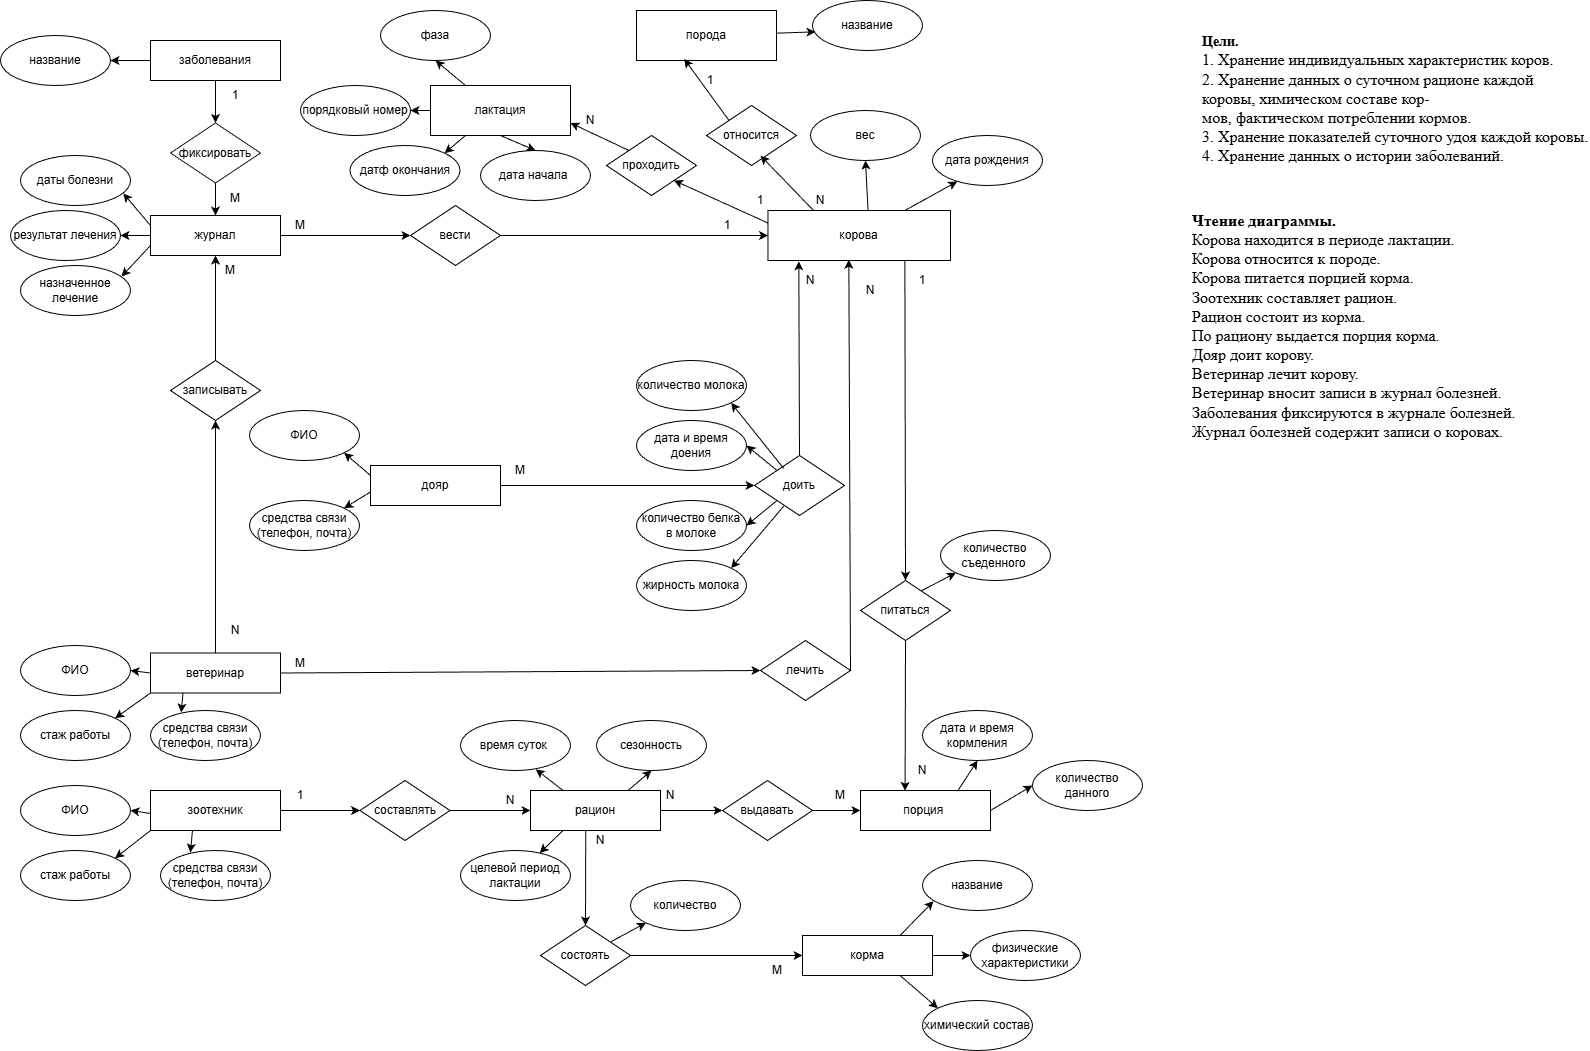
\includegraphics[width=\textwidth, height=\textheight, keepaspectratio]{только er-диаграмма_итог.drawio.png}
        \caption{ER-диаграмма}
        \label{fig:er}
    \end{figure}
\end{landscape}
\restoregeometry
\clearpage
\textbf{Чтение диаграммы.}

\begin{itemize}
    \item Корова находится в периоде лактации.
    \item Корова относится к породе.
    \item Корова питается порцией корма.
    \item Зоотехник составляет рацион.
    \item Рацион состоит из корма.
    \item По рациону выдается порция корма.
    \item Дояр доит корову.
    \item Ветеринар лечит корову.
    \item Ветеринар вносит записи в журнал болезней.
    \item Заболевания фиксируются в журнале болезней.
    \item Журнал болезней содержит записи о коровах.
\end{itemize}

\begin{figure}[H]
    \centering
    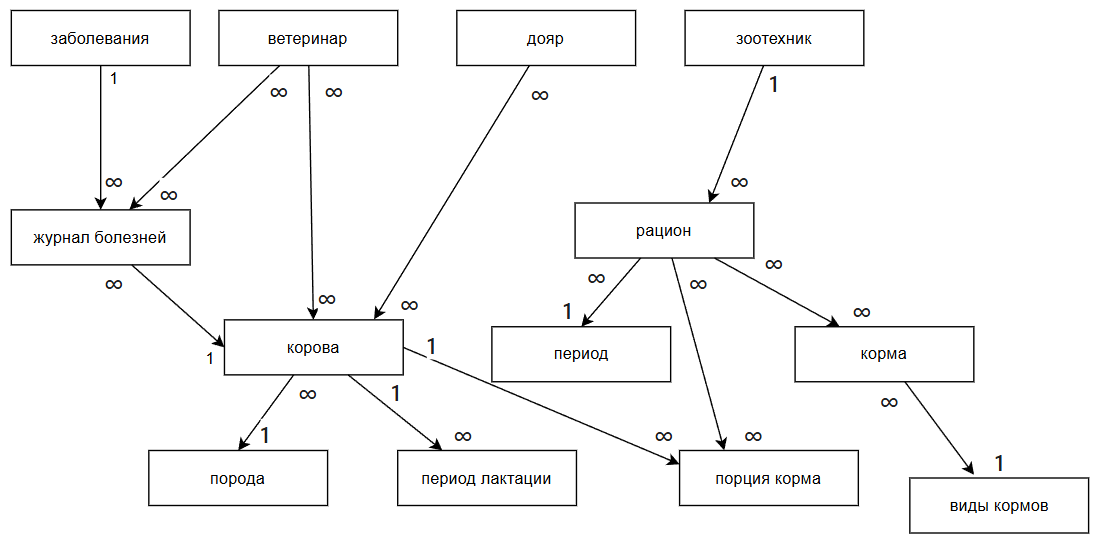
\includegraphics[width=0.75\linewidth]{связи_объектов.png}
    \caption{Схема связи объектов}
    \label{fig:связи_объектов}
\end{figure}